% ============================================================
%  MAIN.TEX — E-Chat Project Report
%  Format: Senior "Passed" Template (Example Report PDF)
%  Font: Times New Roman
%  Body: 12pt, 1.5x line spacing, Justified
%  Margins: Left 1.25in, Right/Top/Bottom 1.0in
% ============================================================
\documentclass[12pt,a4paper,oneside]{report}

% ---- Packages -----------------------------------------------
\usepackage[T1]{fontenc}
\usepackage[utf8]{inputenc}
\usepackage{newtxtext,newtxmath} % Times New Roman for pdfLaTeX

\usepackage[
  a4paper,
  left=1.25in,
  right=1.0in,
  top=1.0in,
  bottom=1.0in
]{geometry}

\usepackage{setspace}
\onehalfspacing

\usepackage{ragged2e}
\setlength{\parindent}{0pt}
\setlength{\parskip}{6pt}

\usepackage{titlesec}
\titleformat{\chapter}[display]
  {\centering\bfseries\fontsize{16}{20}\selectfont}
  {CHAPTER \thechapter}
  {6pt}
  {\MakeUppercase}
\titlespacing*{\chapter}{0pt}{0pt}{18pt}

\titleformat{name=\chapter,numberless}[block]
  {\centering\bfseries\fontsize{14}{18}\selectfont}
  {}
  {0pt}
  {\MakeUppercase}
\titlespacing*{name=\chapter,numberless}{0pt}{0pt}{18pt}

\titleformat{\section}
  {\bfseries\fontsize{14}{18}\selectfont}
  {\thesection}
  {1em}
  {\MakeUppercase}
\titlespacing*{\section}{0pt}{12pt}{6pt}

\titleformat{name=\section,numberless}[block]
  {\bfseries\fontsize{12}{15}\selectfont}
  {}
  {0pt}
  {}
\titlespacing*{name=\section,numberless}{0pt}{10pt}{4pt}

\titleformat{\subsection}
  {\bfseries\fontsize{12}{15}\selectfont}
  {\thesubsection}
  {1em}
  {}
\titlespacing*{\subsection}{0pt}{10pt}{4pt}

\usepackage{graphicx}
\graphicspath{{figures/}}

\usepackage{xcolor}
\usepackage{fancyhdr}
\newcommand{\rupee}{Rs.\ }
\usepackage{caption}
\captionsetup{
  font=normalsize,
  labelfont=normalfont,
  textfont=normalfont,
  labelsep=period,
  justification=centering
}
\captionsetup[table]{position=above}
\captionsetup[figure]{position=below}

\usepackage{tabularx}
\usepackage{longtable}
\usepackage{booktabs}
\usepackage{array}
\newcolumntype{L}[1]{>{\raggedright\arraybackslash}p{#1}}
\newcolumntype{C}[1]{>{\centering\arraybackslash}p{#1}}

\usepackage{enumitem}
\usepackage{amsmath}
\usepackage{amssymb}
\usepackage{float}
\usepackage{listings}
\usepackage{url}

% --- Code listing global style ---
\lstset{
  basicstyle=\ttfamily\small,
  breaklines=true,
  breakatwhitespace=false,
  breakautoindent=true,
  postbreak=\mbox{\textcolor{gray}{$\hookrightarrow$}\space},
  columns=flexible,
  keepspaces=true,
  showstringspaces=false,
  frame=single,
  framesep=4pt,
  xleftmargin=6pt,
  xrightmargin=6pt,
  captionpos=b,
  numbers=none,
  tabsize=4,
}
\usepackage{hyperref}
\hypersetup{
  colorlinks=false,
  hidelinks,
}

% --- Custom TOC Format (Senior Template Style) ---
\usepackage{tocloft}
\renewcommand{\cftchapleader}{\cftdotfill{\cftdotsep}}
\renewcommand{\cftsecleader}{\cftdotfill{\cftdotsep}}
\renewcommand{\cftsubsecleader}{\cftdotfill{\cftdotsep}}
\renewcommand{\cftchapfont}{\bfseries}
\renewcommand{\cftchappagefont}{\bfseries}
\setlength{\cftbeforechapskip}{4pt}
\setlength{\cftbeforesecskip}{1pt}
\setcounter{secnumdepth}{2}
\setcounter{tocdepth}{2}

\makeatletter
\newcommand{\echattableofcontents}{%
  \chapter*{CONTENTS}%
  \phantomsection%
  \label{front:contents}%
  \thispagestyle{plain}%
  \@starttoc{toc}%
}
\newcommand{\echatlistoftables}{%
  \chapter*{LIST OF TABLES}%
  \phantomsection%
  \addcontentsline{toc}{chapter}{LIST OF TABLES}%
  \label{front:lot}%
  \thispagestyle{plain}%
  \@starttoc{lot}%
}
\newcommand{\echatlistoffigures}{%
  \chapter*{LIST OF FIGURES}%
  \phantomsection%
  \addcontentsline{toc}{chapter}{LIST OF FIGURES}%
  \label{front:lof}%
  \thispagestyle{plain}%
  \@starttoc{lof}%
}
\makeatother

% ============================================================

\begin{document}

% ---- Front matter (roman page numbers) ---------------------
\pagenumbering{roman}
\setcounter{page}{1}
\pagestyle{plain}

%% PAGE 1 - Title Page
\begin{titlepage}
\begin{center}

\vspace*{0.8cm}

{\Large\textbf{E-CHAT: A REAL-TIME SECURE WEB-BASED\\[4pt] CHAT APPLICATION}}

\vspace{1.2cm}

{\normalsize MINI PROJECT REPORT}

\vspace{0.5cm}

{\normalsize Submitted by}

\vspace{0.9cm}

\begin{tabular}{p{6cm} p{4cm}}
\textbf{MARVIN M VARGHESE} & \textbf{TKI23CS064} \\[8pt]
\textbf{MUHAMMED SAJID} & \textbf{TKI20CS077} \\[8pt]
\textbf{PARTHAN S} & \textbf{TKI20CS090} \\[8pt]
\textbf{AZEEM N} & \textbf{TKI20CS038} \\
\end{tabular}

\vspace{0.5cm}

{\normalsize To}\\[4pt]
{\normalsize the APJ Abdul Kalam Technological University}\\[4pt]
{\normalsize in partial fulfillment of the requirements for the award of the Degree of}\\[4pt]
{\normalsize Bachelor of Technology in}\\[6pt]
{\normalsize \textit{Computer Science and Engineering}}

\vspace{0.35cm}


\includegraphics[width=5.5cm]{tkm_logo.png}

\vspace{0.25cm}

{\large\textbf{Department of Computer Science and Engineering}}

\vspace{0.35cm}

{\normalsize TKM Institute of Technology}\\[2pt]
{\normalsize Karuvelil, Kollam}

\vspace{0.35cm}

{\large APRIL 2026}

\end{center}
\end{titlepage}

%% PAGE 2 - Declaration
\setcounter{page}{2}
\phantomsection
\addcontentsline{toc}{chapter}{DECLARATION}
\label{front:declaration}
\begin{center}
{\large\textbf{DECLARATION}}
\end{center}

\vspace{1.5cm}

\begin{justify}
We undersigned hereby declare that the project report ``\textbf{E-Chat: A Real-Time Secure Web-Based Chat Application}'' , submitted for partial fulfillment of the requirements for the award of degree of Bachelor of Technology of the APJ Abdul Kalam Technological University, Kerala is a Bonafide work done by us under supervision of Dr. Ajesh F and Dr. Sanila S. This submission represents our ideas in our own words and where ideas or words of others have been included, we have adequately and accurately cited and referenced the original sources. We also declare that we have adhered to ethics of academic honesty and integrity and have not misrepresented or fabricated any data or idea or fact or source in our submission. We understand that any violation of the above will be a cause for disciplinary action by the institute and/or the University and can also evoke penal action from the sources which have thus not been properly cited or from whom proper permission has not been obtained. This report has not been previously formed the basis for the award of any degree, diploma or similar title of any other University.
\end{justify}

\vspace{1.2cm}

Place: Kollam

\vspace{1.5cm}

\begin{flushright}
\textbf{MARVIN M VARGHESE}\\[10pt]
\textbf{MUHAMMED SAJID}\\[10pt]
\textbf{PARTHAN S}\\[10pt]
\textbf{AZEEM N}
\end{flushright}

\newpage

%% PAGE 3 - Certificate
\setcounter{page}{3}
\phantomsection
\addcontentsline{toc}{chapter}{CERTIFICATE}
\label{front:certificate}
\begin{center}
{\large\textbf{DEPARTMENT OF COMPUTER SCIENCE AND ENGINEERING\\[4pt]
TKM INSTITUTE OF TECHNOLOGY, KARUVELIL, KOLLAM}}
\end{center}

\vspace{0.5cm}

\begin{center}

\includegraphics[width=5.5cm]{tkm_logo.png}
\end{center}

\vspace{0.5cm}

\begin{center}
{\large\textbf{CERTIFICATE}}
\end{center}

\vspace{1.2cm}

\begin{justify}
This is to certify that the report entitled ``\textbf{E-Chat: A Real-Time Secure Web-Based Chat Application}'' submitted by \textbf{MARVIN M VARGHESE, MUHAMMED SAJID, PARTHAN S, AZEEM N} to the APJ Abdul Kalam Technological University in partial fulfillment of the requirements for the award of degree of Bachelor of Technology in \textbf{COMPUTER SCIENCE AND ENGINEERING} is a Bonafide record of the project work carried out by them under our guidance and supervision. This report in any form has not been submitted to any other University or Institute for any purpose.
\end{justify}

\vspace{2.5cm}

\noindent
\begin{tabular}{p{4.5cm} p{4.5cm} p{4.5cm}}
Internal Supervisors: & Project Coordinator: & Head of the Dept: \\[6pt]
\textbf{DR. AJESH F} & \textbf{DR. AJESH F} & \textbf{DR. NIJIL RAJ N} \\[4pt]
\textbf{Professor, Dept of CSE} & \textbf{Professor, Dept of CSE} & \textbf{HOD, Dept of CSE} \\[8pt]
\textbf{DR. SANILA S} & & \\
\textbf{Assoc. Prof, Dept of CSE} & & \\
\end{tabular}

\newpage

%% PAGE 4 - Acknowledgement
\phantomsection
\addcontentsline{toc}{chapter}{ACKNOWLEDGEMENT}
\label{front:acknowledgement}
\begin{center}
\textbf{ACKNOWLEDGEMENT}
\end{center}

\vspace{1.5em}

\setlength{\parindent}{0pt}
\setlength{\parskip}{0.8em}

First of all, we thank God Almighty for helping us to successfully complete our project work. We express our sincere thanks and a deep sense of humble gratitude to the Principal of this institution, \textbf{GOURI MOHAN L} ~for providing all the necessary facilities.

We thank \textbf{DR. NIJIL RAJ N}, Head of the Department \& Dean Academics, Computer Science and Engineering, for all the words of inspiration.

Next, we would like to thank our project coordinator \textbf{DR AJESH F} for his valuable advices.

We have great pleasure in expressing our deep sense of gratitude and obligation to our project guides \textbf{DR. AJESH F} and \textbf{DR. SANILA S} for their valuable guidance and suggestions throughout the entire project work.

We also express our sincere thanks to \textbf{Ms. Saina Nazim} for her support, encouragement, and guidance throughout the project.

Last but certainly not the least; We would also like to thank all faculty of Department of Computer Science and Engineering and our friends for their help and co-operation.

\vspace{6em}

\begin{flushright}
\textbf{MARVIN M VARGHESE}\\
\textbf{MUHAMMED SAJID}\\
\textbf{PARTHAN S}\\
\textbf{AZEEM N}
\end{flushright}

\vfill
\begin{center}
  
\end{center}

\newpage
\setlength{\parskip}{6pt}

% ============================================================
%  PREMATTER — Acknowledgement, Abstract, SDG, CO-PO, Feasibility
% ============================================================

% ========================
%  2. ABSTRACT
% ========================
\cleardoublepage
\phantomsection
\addcontentsline{toc}{chapter}{ABSTRACT}
\label{front:abstract}
\thispagestyle{plain}

\begin{center}
{\fontsize{12}{14}\bfseries ABSTRACT\par}
\end{center}

E-Chat is a full-stack real-time communication platform designed and implemented as a web-based application for secure personal and group messaging. The system uses a FastAPI backend with Socket.IO for low-latency bidirectional communication and a Next.js frontend for responsive user interaction across desktop and mobile devices. Core features include JWT-based authentication, contact management, one-to-one and group chat, file sharing, typing indicators, read receipts, message reactions, message edit and delete operations, and call history logging. Browser-based voice and video calling is supported using WebRTC, while Socket.IO is used as the signaling channel for session establishment. The data layer is implemented using asynchronous SQLAlchemy with SQLite/PostgreSQL compatibility to support both development and production deployment. The application also includes profile management and password reset through OTP verification. The modular architecture, use of open-source technologies, and deployability on low-cost cloud platforms make E-Chat technically robust and economically feasible for educational institutions, startups, and small organizations that require a self-hosted and customizable communication solution.

\vspace{0.5cm}
\noindent \textbf{Keywords:} Real-time chat, FastAPI, Socket.IO, Next.js, WebRTC, JWT authentication.

\cleardoublepage

% ========================
%  CONTENTS + LISTS
% ========================
\thispagestyle{plain}
\begingroup
\fontsize{11}{14}\selectfont
\echattableofcontents
\endgroup

\cleardoublepage

\echatlistoftables
\cleardoublepage

\echatlistoffigures
\cleardoublepage

% ========================
%  3. SDG MAPPING
% ========================
\chapter*{SUSTAINABLE DEVELOPMENT GOALS (SDG) MAPPING}
\phantomsection
\addcontentsline{toc}{chapter}{SUSTAINABLE DEVELOPMENT GOALS (SDG) MAPPING}
\label{front:sdg}
\thispagestyle{plain}

The proposed E-Chat project contributes to selected United Nations Sustainable Development Goals by improving communication accessibility, supporting innovation in digital infrastructure, and reducing dependence on high-cost proprietary communication platforms.

\begin{table}[H]
\centering
\caption{SDG Mapping for E-Chat}
\begin{tabularx}{\textwidth}{|C{1.8cm}|C{4.1cm}|X|}
\hline
\textbf{SDG No.} & \textbf{SDG Title} & \textbf{Alignment with E-Chat} \\
\hline
SDG 9 & Industry, Innovation and Infrastructure & E-Chat uses modern software architecture and open standards to build reliable digital communication infrastructure for institutions and teams. \\
\hline
SDG 10 & Reduced Inequalities & Self-hosted and open-source deployment options help reduce access barriers for organizations with limited budgets. \\
\hline
SDG 11 & Sustainable Cities and Communities & Supports connected and collaborative communities through secure and scalable local communication platforms. \\
\hline
\end{tabularx}
\end{table}

\cleardoublepage

% ========================
%  4. COs, POs, CO-PO MAPPING
% ========================
\chapter*{CO-PO MAPPING}
\phantomsection
\addcontentsline{toc}{chapter}{CO-PO MAPPING}
\label{front:copo}
\thispagestyle{plain}

\textbf{Course Outcomes Addressed:}
\begin{enumerate}[leftmargin=1.2cm]
  \item CO1: Identify technically and economically feasible software engineering problems.
  \item CO2: Survey related literature and existing software systems.
  \item CO3: Perform requirement analysis, design, implementation, and testing using modern tools.
  \item CO4: Prepare technical reports and present engineering outcomes.
  \item CO5: Apply engineering and management principles for successful project completion.
\end{enumerate}

\textbf{Program Outcomes Addressed:}
\begin{enumerate}[leftmargin=1.2cm]
  \item PO1: Engineering Knowledge
  \item PO2: Problem Analysis
  \item PO3: Design/Development of Solutions
  \item PO4: Conduct Investigations of Complex Problems
  \item PO5: Modern Tool Usage
  \item PO6: The Engineer and Society
  \item PO7: Environment and Sustainability
  \item PO8: Ethics
  \item PO9: Individual and Team Work
  \item PO10: Communication
  \item PO11: Project Management and Finance
  \item PO12: Lifelong Learning
\end{enumerate}

\begin{table}[H]
\centering
\caption{CO-PO Mapping}
{\fontsize{9}{11}\selectfont
\begin{tabular}{|c|*{12}{c|}}
\hline
\textbf{CO/PO} & \textbf{1} & \textbf{2} & \textbf{3} & \textbf{4} & \textbf{5} & \textbf{6} & \textbf{7} & \textbf{8} & \textbf{9} & \textbf{10} & \textbf{11} & \textbf{12} \\
\hline
CO1 & $\checkmark$ & $\checkmark$ & $\checkmark$ & $\checkmark$ & & $\checkmark$ & $\checkmark$ & $\checkmark$ & $\checkmark$ & $\checkmark$ & $\checkmark$ & $\checkmark$ \\
\hline
CO2 & $\checkmark$ & $\checkmark$ & $\checkmark$ & $\checkmark$ & $\checkmark$ & $\checkmark$ & & $\checkmark$ & $\checkmark$ & $\checkmark$ & $\checkmark$ & $\checkmark$ \\
\hline
CO3 & $\checkmark$ & $\checkmark$ & $\checkmark$ & $\checkmark$ & $\checkmark$ & $\checkmark$ & $\checkmark$ & $\checkmark$ & $\checkmark$ & $\checkmark$ & $\checkmark$ & $\checkmark$ \\
\hline
CO4 & $\checkmark$ & $\checkmark$ & $\checkmark$ & $\checkmark$ & $\checkmark$ & & & $\checkmark$ & $\checkmark$ & $\checkmark$ & $\checkmark$ & $\checkmark$ \\
\hline
CO5 & $\checkmark$ & $\checkmark$ & $\checkmark$ & $\checkmark$ & $\checkmark$ & $\checkmark$ & $\checkmark$ & $\checkmark$ & $\checkmark$ & & $\checkmark$ & $\checkmark$ \\
\hline
\end{tabular}}
\end{table}

\cleardoublepage

% ========================
%  5. TECHNICAL AND ECONOMIC FEASIBILITY
% ========================
\chapter*{TECHNICAL AND ECONOMIC FEASIBILITY}
\phantomsection
\addcontentsline{toc}{chapter}{TECHNICAL AND ECONOMIC FEASIBILITY}
\label{front:feasibility}
\thispagestyle{plain}

\section*{1. TECHNICAL FEASIBILITY}
\addcontentsline{toc}{section}{1. TECHNICAL FEASIBILITY}
\label{front:technical-feasibility}
The proposed E-Chat system is technically feasible because it is implemented using stable and widely adopted technologies: FastAPI, Socket.IO, SQLAlchemy, and Next.js. The required software stack is open source, well documented, and compatible with standard development machines. No specialized hardware is required for development or deployment. The architecture supports modular expansion, making future enhancements such as distributed messaging and TURN relay integration practical.

\section*{2. ECONOMIC FEASIBILITY}
\addcontentsline{toc}{section}{2. ECONOMIC FEASIBILITY}
\label{front:economic-feasibility}
The project is economically feasible for academic and small-scale industry adoption. Development uses free and open-source tools. Deployment can be done on affordable cloud instances with low recurring cost. Since the platform is self-hostable, organizations can avoid recurring per-user subscription charges of proprietary collaboration software. Therefore, the total ownership cost remains low while retaining customizability and data control.

\cleardoublepage

% ========================
%  ABBREVIATIONS
% ========================
\chapter*{ABBREVIATIONS}
\phantomsection
\addcontentsline{toc}{chapter}{ABBREVIATIONS}
\label{front:abbreviations}
\thispagestyle{plain}

\begin{tabularx}{\textwidth}{@{}L{3cm}X@{}}
API & Application Programming Interface \\
ASGI & Asynchronous Server Gateway Interface \\
DB & Database \\
JWT & JSON Web Token \\
OTP & One-Time Password \\
P2P & Peer-to-Peer \\
RTT & Round Trip Time \\
SDP & Session Description Protocol \\
STUN & Session Traversal Utilities for NAT \\
TURN & Traversal Using Relays around NAT \\
UI & User Interface \\
WebRTC & Web Real-Time Communication \\
\end{tabularx}

\cleardoublepage

% ========================
%  NOTATION
% ========================
\chapter*{NOTATION}
\phantomsection
\addcontentsline{toc}{chapter}{NOTATION}
\label{front:notation}
\thispagestyle{plain}

\begin{tabularx}{\textwidth}{@{}L{3cm}X@{}}
$u$ & Number of active users connected to the system \\
$m$ & Number of messages exchanged in a conversation \\
$t_{rtt}$ & Message round-trip latency (ms) \\
$S_{msg}$ & Size of message payload (bytes) \\
$C_{max}$ & Maximum concurrent users supported per node \\
$C_{deploy}$ & Monthly deployment cost (\rupee/month) \\
\end{tabularx}

\cleardoublepage

% ---- Main matter (arabic page numbers) ---------------------
\pagenumbering{arabic}

% ============================================================
%  CHAPTER 1 — INTRODUCTION
%  Template: Senior "Passed" Report
% ============================================================
\chapter{INTRODUCTION}
\label{chap:introduction}
\thispagestyle{plain}

\section{Background and Context}
\label{sec:background-context}

The rapid evolution of digital communication has transformed how individuals and
organizations interact. Real-time messaging, once a luxury, is now a fundamental
requirement for personal and professional collaboration. E-Chat is a secure,
self-hostable web-based chat application designed to provide a privacy-focused
alternative to centralized messaging services.

\section{Problem Statement}
\label{sec:problem-statement}

Current centralized messaging platforms often face challenges regarding data
privacy, high subscription costs, and lack of customization for organizational
needs. Many proprietary systems also lack transparency in how user data is
processed and stored. Many open-source alternatives provide only partial feature
coverage or require significant customization before they can support direct
messaging, group communication, file exchange, and browser-based calling in a
single workflow.

\section{Objectives}
\label{sec:objectives}
The primary objectives of the E-Chat project include:
\begin{enumerate}
    \item To build a real-time messaging platform using Socket.IO.
    \item To implement secure authentication using JWT and password hashing.
    \item To provide browser-based audio and video communication via WebRTC signaling.
    \item To ensure cost-effective and portable cloud deployment.
\end{enumerate}

\section{Scope and Limitations}
\label{sec:scope-limitations}
Existing chat solutions frequently require high bandwidth and specialized hardware
for self-hosted environments. Additionally, the lack of real-time multi-media
capabilities in most open-source chat frameworks limits their utility for modern
workplaces.

The scope of this project includes user authentication, contact-based communication,
group chat, file sharing, and WebRTC call signaling. End-to-end encryption and
distributed multi-node message brokering are outside the current implementation scope.

\section{Industry Relevance}
\label{sec:industry-relevance}

The project addresses current industrial trends and needs:
\begin{itemize}
    \item \textbf{High Demand for Secure Communication:} The increasing reliance on remote
          work and digital collaboration in the IT industry makes secure, private
          communication tools critical for protecting intellectual property.
    \item \textbf{Open-Source Cost Efficiency:} Many organizations are moving away
          from expensive SaaS subscriptions (like Slack or Teams) toward open-source
          or self-hosted solutions to reduce operational costs.
    \item \textbf{Real-Time API Ecosystem:} The use of WebSockets and FastAPI is
          highly relevant to modern software development, where low-latency API
          delivery is essential.
    \item \textbf{Scalable Web Architecture:} E-Chat demonstrates the implementation
          of a production-ready full-stack application that integrates complex
          real-time workflows (WebRTC and Socket.IO), which is a key requirement
          in the modern tech landscape.
\end{itemize}

\section{Proposed System}
\label{sec:proposed-system}

The proposed system, E-Chat, implements a modular architecture to address the
limitations of existing solutions:

\subsection{Core Messaging}
\label{subsec:core-messaging}
The system uses a Python-based Socket.IO backend to handle direct messaging,
group messaging, typing events, read receipts, and live status updates with
low latency and efficient event routing.

\subsection{Media Communication}
\label{subsec:media-communication}
E-Chat integrates browser-native WebRTC to support audio and video calls. The
signaling flow is managed through Socket.IO, allowing peers to exchange offer,
answer, and ICE candidate data before the media path is established.

\subsection{Security Design}
\label{subsec:security-design}
The application employs JWT-based authentication, hashed password storage, and
protected API endpoints. File uploads and profile operations are authenticated,
and the architecture is designed to support secure self-hosted deployment.

\subsection{User Interface}
\label{subsec:user-interface}
The frontend is built with Next.js and TypeScript to provide a responsive and
modern user experience across desktops and mobile devices. The chat interface,
settings views, attachment rendering, and AI chat area are implemented with a
consistent component-driven design.

\section{Organization of the Report}
\label{sec:organization-report}
This report is organized into seven chapters. Chapter 1 introduces the project
background, problem statement, objectives, and relevance. Chapter 2 reviews
existing work in real-time communication systems and identifies gaps. Chapter 3
describes the methodology, architecture, and data model. Chapter 4 presents the
project plan and team responsibilities. Chapter 5 documents implementation,
block diagrams, and testing. Chapter 6 presents the obtained results, their
analysis, and key limitations. Chapter 7 concludes with future directions and
practical application areas of the system.

\cleardoublepage

% ============================================================
%  CHAPTER 2 — REVIEW OF LITERATURE
% ============================================================
\chapter{REVIEW OF LITERATURE}
\label{chap:literature}
\thispagestyle{plain}

\section{Summary of Existing Work}
\label{sec:existing-work}

Real-time communication systems have evolved from HTTP polling to persistent
socket-based communication. WebSocket protocol standards enabled low-latency
bi-directional messaging, while frameworks such as Socket.IO improved reliability
through reconnection and fallback mechanisms. In parallel, WebRTC introduced
browser-native audio and video communication through peer-to-peer channels.

Modern backend frameworks such as FastAPI and asynchronous Python runtimes
improved the practicality of handling high numbers of long-lived connections.
On the client side, React and Next.js enabled component-based, highly responsive
interfaces suitable for dynamic chat windows, typing indicators, and live status.

\section{Real-Time Messaging Platforms}
\label{sec:messaging-platforms}
Real-time messaging platforms generally combine persistent communication channels,
user session management, and message persistence. Enterprise-grade solutions such
as Slack, Microsoft Teams, and Discord demonstrate the importance of low-latency
transport, rich client interfaces, and multi-device synchronization. However,
these systems are primarily cloud-hosted and subscription oriented.

Open-source alternatives provide more control and extensibility, but many focus
either on messaging alone or on large self-hosted ecosystems that are harder to
adapt for a focused academic implementation. This creates room for a modular
project like E-Chat that demonstrates modern communication features in a smaller
and more understandable system.

\section{Security Practices in Communication Systems}
\label{sec:security-practices}
Security in communication systems is not limited to transport encryption. It also
involves secure authentication, robust password storage, controlled access to
attachments, protected profile operations, and resilient session handling.
Current best practices recommend adaptive password hashing, token-based access,
server-side validation of all privileged actions, and minimal exposure of user data.

These principles directly influence the design of E-Chat. The system uses JWT
authentication, protected APIs, and bounded file-upload handling. Even though the
current project does not yet implement end-to-end encryption, its present security
layer provides a meaningful foundation for safe institutional deployment.

\section{Gaps Identified}
\label{sec:gaps-identified}

Despite major advances, many existing communication platforms show one or more
of the following limitations:
\begin{itemize}
  \item Strong dependence on centralized proprietary infrastructure.
  \item Limited customization for institution-specific workflows.
  \item High recurring licensing cost for per-user subscriptions.
  \item Incomplete integration of messaging, media calls, and profile management in lightweight academic projects.
  \item Weak support for self-hosting and transparent control over stored user data.
\end{itemize}

\section{Contribution of E-Chat}
\label{sec:echat-contribution}

E-Chat addresses the identified gaps by combining open-source technologies into
a unified and deployable product:
\begin{itemize}
  \item FastAPI + Socket.IO backend for secure, event-driven real-time messaging.
  \item Next.js frontend with responsive UI for desktop and mobile usage.
  \item Built-in WebRTC call signaling for voice and video communication.
  \item User profile management, read receipts, reactions, and file sharing in one platform.
  \item Self-hostable architecture suitable for academic institutions and small organizations.
\end{itemize}

\section{Concluding Remarks}
\label{sec:literature-conclusion}

The literature supports the technical viability of event-driven communication
systems. The E-Chat project extends this foundation into an integrated, practical,
and low-cost communication platform aligned with current industry trends.

\cleardoublepage

% ============================================================
%  CHAPTER 3 — METHODOLOGY / THEORY / MODELLING
% ============================================================
\chapter{METHODOLOGY / THEORY / MODELLING}
\label{chap:methodology}
\thispagestyle{plain}

\section{Approach}
\label{sec:approach}

The E-Chat project follows an iterative full-stack development process with
short implementation and validation cycles. The architecture is designed in
three logical layers:
\begin{itemize}
  \item \textbf{Presentation Layer:} Next.js user interface and client state handling.
  \item \textbf{Communication Layer:} Socket.IO event routing for real-time messaging and signaling.
  \item \textbf{Data Layer:} FastAPI + SQLAlchemy async persistence model.
\end{itemize}

\section{Theoretical Framework}
\label{sec:theoretical-framework}

\subsection{Event-Driven Communication Model}
\label{subsec:event-driven-model}
Conventional request-response messaging is not sufficient for real-time chat.
E-Chat uses an event-driven model where each connected session is authenticated
with JWT and mapped to a user identity. Messages are emitted to user-specific
sessions, enabling fast delivery and acknowledgements.

\subsection{WebRTC Signaling Model}
\label{subsec:webrtc-signaling}
WebRTC calls are established with the offer-answer flow:
\begin{enumerate}
  \item Caller creates and sends SDP offer through Socket.IO.
  \item Callee receives the offer and sends SDP answer.
  \item ICE candidates are exchanged.
  \item Peer-to-peer media path is established.
\end{enumerate}

\subsection{Authentication and Password Security}
\label{subsec:password-security}
E-Chat uses JWT for stateless authentication and password hashing using bcrypt
with SHA-256 pre-hash at application level:
\[
\text{Stored Password} = \text{bcrypt}(\text{sha256}(\text{password}))
\]
This structure improves resistance against straightforward credential disclosure.

\section{Tools and Technologies}
\label{sec:tools-technologies}

\begin{itemize}
  \item \textbf{Backend:} FastAPI, python-socketio, SQLAlchemy Async, PostgreSQL/SQLite.
  \item \textbf{Frontend:} Next.js, React, TypeScript, Zustand, Tailwind CSS.
  \item \textbf{Communication:} Socket.IO, WebRTC.
  \item \textbf{Deployment:} Docker and cloud deployment descriptors for multiple platforms.
  \item \textbf{Versioning and Collaboration:} GitHub-based source management and issue tracking.
\end{itemize}

\section{System Architecture Model}
\label{sec:system-architecture-model}
The E-Chat architecture follows a layered full-stack model. The frontend handles
user interaction, page routing, and local state synchronization. The backend
provides REST APIs for authentication, profile access, contact management, file
upload, and message history. Socket.IO is used alongside the REST layer to manage
real-time events such as new messages, message acknowledgements, typing state,
status updates, and call signaling.

This dual-channel model is important because it improves resilience. Users can
continue core actions through HTTP even when real-time delivery is temporarily
interrupted. The architecture therefore balances responsiveness with operational
reliability.

\begin{figure}[H]
    \centering
    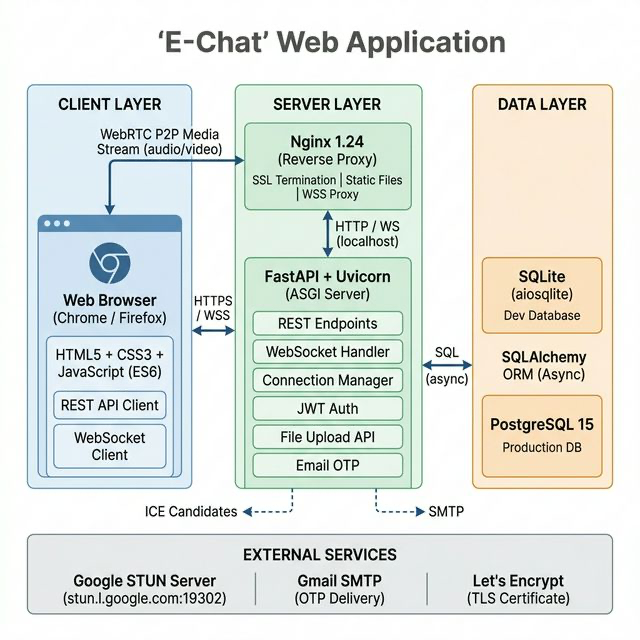
\includegraphics[width=0.88\textwidth]{system_architecture.png}
    \caption{Overall system architecture of E-Chat showing frontend, backend, database, and real-time communication layers.}
    \label{fig:system_architecture_methodology}
\end{figure}

\section{Database Model}
\label{sec:database-model}
The relational data model centers around the \textbf{User} entity and extends into
communication-specific entities such as \textbf{Contact}, \textbf{Group},
\textbf{GroupMember}, and \textbf{Message}. Additional tables such as
\textbf{OTP} and \textbf{CallHistory} support auxiliary workflows. The message
entity is flexible enough to support text, file metadata, status updates, and
emoji reactions.

The database design intentionally avoids unnecessary complexity while supporting
the core features expected from a modern communication platform. This makes it
well suited for both academic demonstration and future extension.

\section{Design Process}
\label{sec:design-process}

The design process started with use-case analysis for chat, contacts, and calling.
Database entities (User, Message, Contact, Group, GroupMember, OTP, CallHistory)
were modeled first, followed by REST endpoint design and event-contract design.
After backend stabilization, the frontend integrated optimistic UI updates,
message status synchronization, and fallback messaging over HTTP. The logical
sequence of a direct message event is shown in Figure~\ref{fig:message_flow},
while the broader system architecture is illustrated earlier in Figure~\ref{fig:system_architecture_methodology}.

\begin{figure}[H]
    \centering
    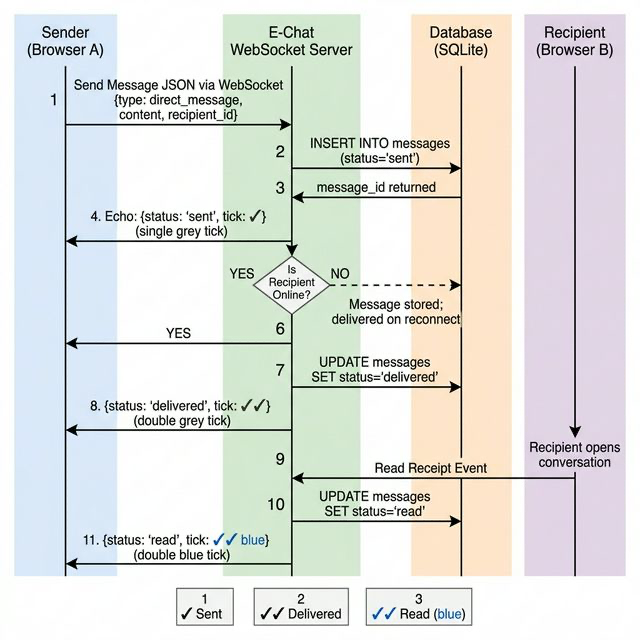
\includegraphics[width=0.85\textwidth]{message_flow.png}
    \caption{Message flow between frontend, Socket.IO layer, and persistence layer.}
    \label{fig:message_flow}
\end{figure}

\cleardoublepage

% ============================================================
%  CHAPTER 4 — WORK PLAN & TASK ALLOCATION
%  Template: Senior "Passed" Report
% ============================================================
\chapter{WORK PLAN AND TASK ALLOCATION}
\label{chap:workplan}
\thispagestyle{plain}

\section{Project Timeline}
\label{sec:project-timeline}

The development was divided into five distinct sprints over ten weeks. The
timeline is presented in Table~\ref{tab:timeline}.

\begin{table}[H]
\centering
\caption{E-Chat Project Timeline}
\label{tab:timeline}
\begin{tabularx}{\textwidth}{|L{2.5cm}|C{3cm}|X|}
\hline
\textbf{Phase} & \textbf{Duration} & \textbf{Tasks} \\
\hline
Sprint 1 & Weeks 1--2 & Requirement analysis, tech selection, and environment setup. \\
\hline
Sprint 2 & Weeks 3--4 & Backend setup (FastAPI), authentication, and database schema. \\
\hline
Sprint 3 & Weeks 5--6 & Core messaging engine (Socket.IO) and group chat logic. \\
\hline
Sprint 4 & Weeks 7--8 & WebRTC integration for voice/video calling and file uploads. \\
\hline
Sprint 5 & Weeks 9--10 & UI refinement, testing, and cloud deployment. \\
\hline
\end{tabularx}
\end{table}

\section{Task Allocation}
\label{sec:task-allocation}

The responsibilities were divided among the four team members based on their
technical strengths and roles:

\begin{itemize}
    \item \textbf{Marvin M Varghese (TKI23CS064):} Backend Lead and Overall Architecture.
          Focused on FastAPI, Socket.IO core messaging, and WebRTC signaling.
    \item \textbf{Muhammed Sajid (TKI20CS077):} Frontend Lead. Responsible for UI
          design, Socket.IO client integration, and real-time state management.
    \item \textbf{Parthan S (TKI20CS090):} Database and Security Lead. Managed the
          database architecture, JWT authentication, and bcrypt hashing layer.
    \item \textbf{Azeem N (TKI20CS038):} Testing and Documentation. Responsible for
          test case design, experimental validation, and technical documentation.
\end{itemize}

\section{Collaboration Tools}
\label{sec:collaboration-tools}

The team used the following tools for effective project management and collaboration:
\begin{itemize}
    \item \textbf{Version Control:} GitHub for code repository and pull requests.
    \item \textbf{Communication:} Slack and Discord for real-time coordination.
    \item \textbf{API Testing:} Postman and Insomnia for validating REST endpoints.
    \item \textbf{Documentation:} LaTeX (pdfLaTeX) for final thesis report writing.
    \item \textbf{Issue Tracking:} GitHub Issues for bug reporting and task management.
\end{itemize}

\section{Milestones and Deliverables}
\label{sec:milestones-deliverables}
The project was managed through milestone-based development. Core milestones
included authentication completion, direct messaging, group chat, profile
management, file upload support, WebRTC signaling, and report preparation.
Each milestone was associated with a concrete deliverable such as a working
module, deployment-ready configuration, architecture diagram, or tested user flow.

This milestone structure improved visibility into progress and helped the team
balance implementation effort with documentation and validation activities.

\cleardoublepage

% ============================================================
%  CHAPTER 5 — EXPERIMENTAL DESIGN / CODING / BLOCK DIAGRAM
% ============================================================
\chapter{EXPERIMENTAL DESIGN / CODING / BLOCK DIAGRAM}
\label{chap:experimental}
\thispagestyle{plain}

% ─────────────────────────────────────────────
\section{Experimental Setup}
\label{sec:experimental-setup}

The experimental evaluation of E-Chat was conducted in a controlled local
development environment as well as over a standard Wi-Fi network, using two
or more browser clients running simultaneously. The backend was executed
using Uvicorn as the ASGI server, and the frontend was served by the Next.js
development server. Both were run on the same machine during initial testing,
and later verified across two devices on the same local area network to
confirm real-time event propagation.

Testing covered the following dimensions:
\begin{itemize}
  \item \textbf{Functional correctness:} All user-facing features were exercised through
        manual browser interaction, including signup, chat, file upload, group messaging,
        call signaling, and profile updates.
  \item \textbf{Event-level validation:} Individual Socket.IO events were inspected
        using browser DevTools and server-side logging to verify proper delivery,
        ordering, and session handling.
  \item \textbf{Network condition testing:} Message exchange was tested on localhost,
        local Wi-Fi, and over a public VPS to measure round-trip latency
        characteristics.
  \item \textbf{Mobile compatibility:} The frontend was validated on both desktop
        (Chrome, Firefox) and mobile browsers to verify responsive layout behavior
        and call screen usability.
\end{itemize}

% ─────────────────────────────────────────────
\section{Coding Details}
\label{sec:coding-details}

This section presents core implementation excerpts from both the backend and
frontend layers. Each excerpt is selected to illustrate a distinct technical
mechanism used in the E-Chat system.

% ---
\subsection{Authentication and Password Security}
\label{subsec:auth-impl}

Authentication in E-Chat is handled by the \texttt{auth.py} module. Passwords
are hardened using a two-stage hashing strategy: the plaintext password is
first transformed with SHA-256, and the resulting digest is then passed through
bcrypt, which automatically appends a random salt. This design prevents bcrypt's
72-byte input limit from silently truncating long passwords, a vulnerability
documented in OWASP password storage guidelines.

\begin{lstlisting}[language=Python, caption=Password Hashing and Verification (auth.py)]
def get_password_hash(password: str) -> str:
    # Stage 1: SHA-256 pre-hash to handle arbitrary length
    sha256 = hashlib.sha256(password.encode("utf-8")).hexdigest()
    # Stage 2: bcrypt with auto-generated salt
    hashed = bcrypt.hashpw(sha256.encode("utf-8"), bcrypt.gensalt())
    return hashed.decode("utf-8")

def verify_password(plain_password: str, hashed_password: str) -> bool:
    sha256 = hashlib.sha256(plain_password.encode("utf-8")).hexdigest()
    return bcrypt.checkpw(
        sha256.encode("utf-8"),
        hashed_password.encode("utf-8")
    )
\end{lstlisting}

JWT tokens are issued on login and signup using the \texttt{python-jose} library.
The token payload carries the user's email (as \texttt{sub}) and numeric ID,
allowing both identity lookup and protected-route authorization without a
database round-trip on every request.

\begin{lstlisting}[language=Python, caption=JWT Token Creation and Verification (auth.py)]
def create_access_token(data: dict,
                        expires_delta: Optional[timedelta] = None) -> str:
    to_encode = data.copy()
    expire = datetime.now(timezone.utc) + (
        expires_delta or timedelta(minutes=15)
    )
    to_encode.update({"exp": expire})
    return jwt.encode(to_encode, SECRET_KEY, algorithm=ALGORITHM)

def verify_token(token: str):
    try:
        payload = jwt.decode(token, SECRET_KEY, algorithms=[ALGORITHM])
        if payload.get("sub") is None:
            return None
        return payload
    except JWTError:
        return None
\end{lstlisting}

The OTP-based password reset flow generates a 6-digit code, stores it with an
expiry timestamp in the \texttt{OTP} table, and dispatches the code via SMTP
asynchronously using \texttt{asyncio.create\_task} so that the HTTP response
is not delayed by the email delivery operation.

% ---
\subsection{Backend Socket.IO Event Handling}
\label{subsec:backend-event-handling}

The Socket.IO server is set up in \texttt{chat\_manager.py} using
\texttt{python-socketio}'s async server interface. A JWT token must be
provided in the Socket.IO handshake auth data. On successful authentication
the server maps the session ID (\texttt{sid}) to the corresponding user ID
in two in-memory dictionaries: \texttt{active\_connections} and
\texttt{session\_to\_user}. These mappings allow the server to address
messages to specific users regardless of how many browser tabs are open.

\begin{lstlisting}[language=Python, caption=Socket.IO Connection and Session Mapping (chat\_manager.py)]
active_connections: Dict[int, Set[str]] = {}
session_to_user: Dict[str, int] = {}

@sio.event
async def connect(sid, environ, auth_data):
    token = auth_data.get("token")
    user = auth.verify_token(token)
    if not user:
        return False          # Reject unauthenticated connections
    user_id = user["id"]
    if user_id not in active_connections:
        active_connections[user_id] = set()
    active_connections[user_id].add(sid)
    session_to_user[sid] = user_id
    await sio.emit("connected", {"user_id": user_id}, room=sid)
    await broadcast_user_status(sio, user_id, "online")
    return True
\end{lstlisting}

When a user sends a message through the socket, the \texttt{send\_message}
handler persists the message to the database through the async CRUD layer and
then dispatches it to the target user's active sessions. If the sender included
a \texttt{\_tempId} field (from the frontend's optimistic rendering logic), the
server echoes it back in the confirmation payload so the frontend can match and
replace the temporary bubble with the server-confirmed record.

\begin{lstlisting}[language=Python, caption=Message Send Handler with Optimistic ID Reconciliation]
@sio.event
async def send_message(sid, data):
    user_id = session_to_user[sid]
    async with database.SessionLocal() as db:
        message = await crud.create_message(
            db,
            sender_id=user_id,
            receiver_id=data.get("receiver_id"),
            group_id=data.get("group_id"),
            content=data.get("content"),
            file_url=data.get("file_url"),
            file_type=data.get("file_type"),
            file_name=data.get("file_name"),
            file_size=data.get("file_size"),
        )
        payload = {
            "id": message.id,
            "content": message.content,
            "sender_id": message.sender_id,
            "receiver_id": message.receiver_id,
            "group_id": message.group_id,
            "created_at": message.created_at.isoformat(),
            "status": message.status,
            "file_url": message.file_url,
            "file_type": message.file_type,
            "file_name": message.file_name,
        }
        if "_tempId" in data:
            payload["_tempId"] = data["_tempId"]
        # Route to recipient(s)
        if message.group_id:
            members = await crud.get_group_members_ids(db, message.group_id)
            for mid in members:
                if mid != user_id:
                    await send_to_user(sio, mid, "new_message", payload)
        elif message.receiver_id:
            await send_to_user(sio, message.receiver_id, "new_message", payload)
        # Confirm to sender
        await sio.emit("message_sent", payload, room=sid)
\end{lstlisting}

% ---
\subsection{Reaction Toggle with JSON Column Management}
\label{subsec:reaction-impl}

Message reactions are stored in the \texttt{reactions} JSON column of the
\texttt{Message} table. Each emoji key maps to a list of user IDs who have
reacted. The toggle logic adds the user if absent or removes them if already
present, then clears the key entirely if the list becomes empty.
A \texttt{flag\_modified} call is required to inform SQLAlchemy that a JSON
column has changed in-place, because the ORM does not track nested mutations
automatically.

\begin{lstlisting}[language=Python, caption=Reaction Toggle in CRUD Layer (crud.py)]
async def toggle_reaction(db: AsyncSession,
                          message_id: int, user_id: int, emoji: str):
    result = await db.execute(
        select(models.Message).where(models.Message.id == message_id)
    )
    message = result.scalars().first()
    if not message:
        return None
    reactions: dict = dict(message.reactions or {})
    users = reactions.get(emoji, [])
    if user_id in users:
        users.remove(user_id)
    else:
        users.append(user_id)
    if users:
        reactions[emoji] = users
    elif emoji in reactions:
        del reactions[emoji]
    message.reactions = reactions
    from sqlalchemy.orm.attributes import flag_modified
    flag_modified(message, "reactions")
    await db.commit()
    await db.refresh(message)
    return message
\end{lstlisting}

% ---
\subsection{Message Edit and Delete}
\label{subsec:edit-delete}

Both edit and delete operations are sender-restricted. The \texttt{edit\_message}
CRUD function verifies that the requesting user is the original sender before
updating the content and setting the \texttt{edited} flag to \texttt{True}.
The delete operation performs a hard removal from the database. After persistence,
the socket layer broadcasts a \texttt{message\_edited} or \texttt{message\_deleted}
event to the relevant participants so all clients reflect the change instantly.

\begin{lstlisting}[language=Python, caption=Message Edit and Delete (crud.py)]
async def edit_message(db, message_id, sender_id, new_content):
    message = await get_message_by_id(db, message_id)
    if not message or message.sender_id != sender_id:
        return None
    message.content = new_content
    message.edited = True
    await db.commit()
    await db.refresh(message)
    return message

async def delete_message(db, message_id, sender_id):
    message = await get_message_by_id(db, message_id)
    if not message or message.sender_id != sender_id:
        return False
    await db.execute(
        sql_delete(models.Message).where(models.Message.id == message_id)
    )
    await db.commit()
    return True
\end{lstlisting}

% ---
\subsection{Frontend Message Dispatch with Optimistic Rendering}
\label{subsec:frontend-message-dispatch}

On the frontend, messages are rendered immediately using a temporary in-memory
record before the server acknowledgement arrives. This is called optimistic
rendering and it eliminates the perceptible delay that would otherwise appear
between a user pressing send and seeing the message appear in the thread. A
negative timestamp is used as the temporary ID to ensure it cannot collide with
real database IDs.

\begin{lstlisting}[language=JavaScript, caption=Optimistic Message Rendering (Frontend)]
const tempId = -Date.now();
// Immediately insert a "sending" bubble into the local state
addMessage({
  id: tempId,
  content: inputText,
  sender_id: currentUser.id,
  status: "sending",
  created_at: new Date().toISOString(),
});
// Dispatch to server with the temp ID
socket.emit("send_message", {
  content: inputText,
  receiver_id: activeContactId,
  _tempId: tempId,
});
// On receiving "message_sent", replace the temporary record
socket.on("message_sent", (confirmed) => {
  replaceMessage(confirmed._tempId, confirmed);
});
\end{lstlisting}

% ---
\subsection{WebRTC Peer Connection and Signaling}
\label{subsec:webrtc-impl}

The WebRTC peer connection is created in the \texttt{CallScreen} component.
Google's public STUN servers are used for ICE candidate gathering. All tracks
from the local media stream are added to the peer connection, and the
\texttt{ontrack} handler attaches incoming remote tracks to a \texttt{MediaStream}
object that feeds both a video element and a separate audio element for reliable
playback. To handle timing issues where ICE candidates arrive before the remote
description is set, incoming candidates are queued and drained once the
signaling state reaches stable.

\begin{lstlisting}[language=JavaScript, caption=WebRTC Setup and ICE Candidate Queuing (call-screen.tsx)]
const STUN_SERVERS = {
  iceServers: [
    { urls: "stun:stun.l.google.com:19302" },
    { urls: "stun:stun1.l.google.com:19302" },
  ]
}
const iceCandidateQueue = useRef([])

const pc = new RTCPeerConnection(STUN_SERVERS)
stream.getTracks().forEach(track => pc.addTrack(track, stream))

pc.ontrack = (e) => {
  e.streams[0]?.getTracks().forEach(t => remoteStream.addTrack(t))
  attachRemoteStream()   // attach to <video> and <audio> elements
  if (e.track.kind === "audio") setConnected(true)
}

pc.onsignalingstatechange = async () => {
  if (pc.signalingState !== "stable") return
  // Drain queued ICE candidates once remote description is applied
  for (const c of iceCandidateQueue.current) {
    await pc.addIceCandidate(new RTCIceCandidate(c)).catch(() => {})
  }
  iceCandidateQueue.current = []
}

// Outgoing call: create offer
const offer = await pc.createOffer({ offerToReceiveAudio: true,
                                     offerToReceiveVideo: isVideo })
await pc.setLocalDescription(offer)
socketService.initiateCall(peerId, callType, offer)

// Incoming call: set remote and answer
await pc.setRemoteDescription(incomingOffer)
const answer = await pc.createAnswer()
await pc.setLocalDescription(answer)
socketService.sendAnswer(callerId, answer)
\end{lstlisting}

% ─────────────────────────────────────────────
\section{Block Diagram and Process Flow}
\label{sec:block-diagram}

The runtime behavior of E-Chat can be understood through the overall system
architecture and the message and call signaling flow diagrams.
Figure~\ref{fig:system_architecture} illustrates the full-stack layering,
showing how the Next.js client communicates with the FastAPI backend over both
REST HTTP and the Socket.IO persistent channel, and how the backend interfaces
with the SQLAlchemy database layer.
Figure~\ref{fig:webrtc_flow} shows the signaling path required to establish
a browser-based WebRTC call, including the offer-answer exchange and ICE
candidate relay managed by the Socket.IO layer.

\begin{figure}[H]
    \centering
    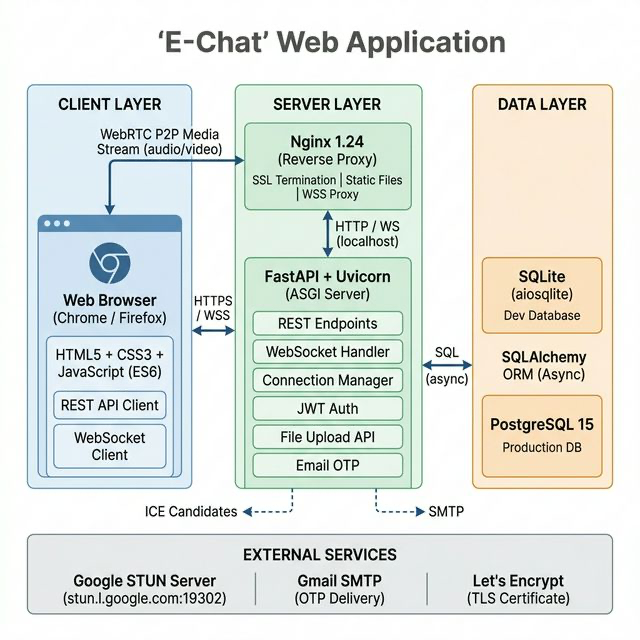
\includegraphics[width=0.88\textwidth]{system_architecture.png}
    \caption{Overall layered architecture of E-Chat showing the frontend, REST
             API, Socket.IO real-time channel, and database persistence components.}
    \label{fig:system_architecture}
\end{figure}

\begin{figure}[H]
    \centering
    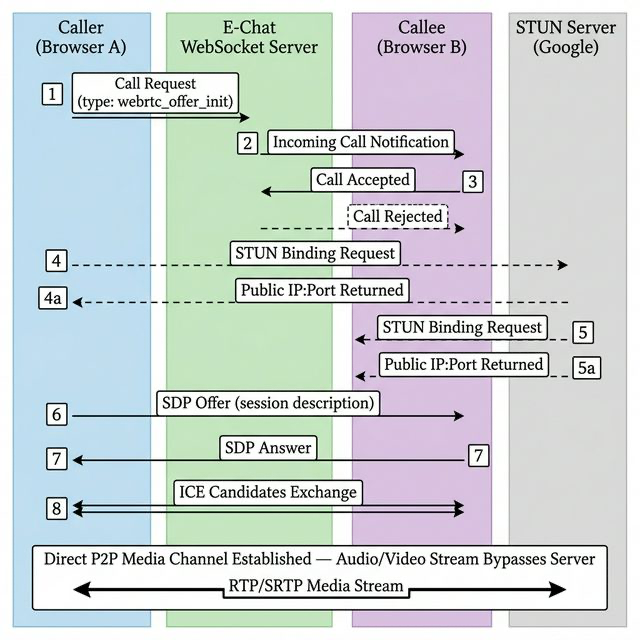
\includegraphics[width=0.88\textwidth]{webrtc_flow.png}
    \caption{WebRTC signaling flow for establishing browser-to-browser audio
             and video calls via the Socket.IO relay server.}
    \label{fig:webrtc_flow}
\end{figure}

% ─────────────────────────────────────────────
\section{Application Screenshots}
\label{sec:app-screenshots}

This section presents screenshots of the implemented E-Chat application to
demonstrate the functional correctness and visual quality of the user interface.
Each screen represents a distinct workflow in the system.

\subsection{Login and Registration}
\label{subsec:screenshot-login}

The signup page collects the user's email and password, validates the input on
the client side, and creates an account via the \texttt{POST /auth/signup}
endpoint. On success, a JWT is returned and the user is redirected to the main
chat view. The login page performs the same token exchange for returning users.
The forgot-password flow extends this screen by triggering an OTP to the
registered email and presenting a reset form after verification.

\begin{figure}[H]
    \centering
    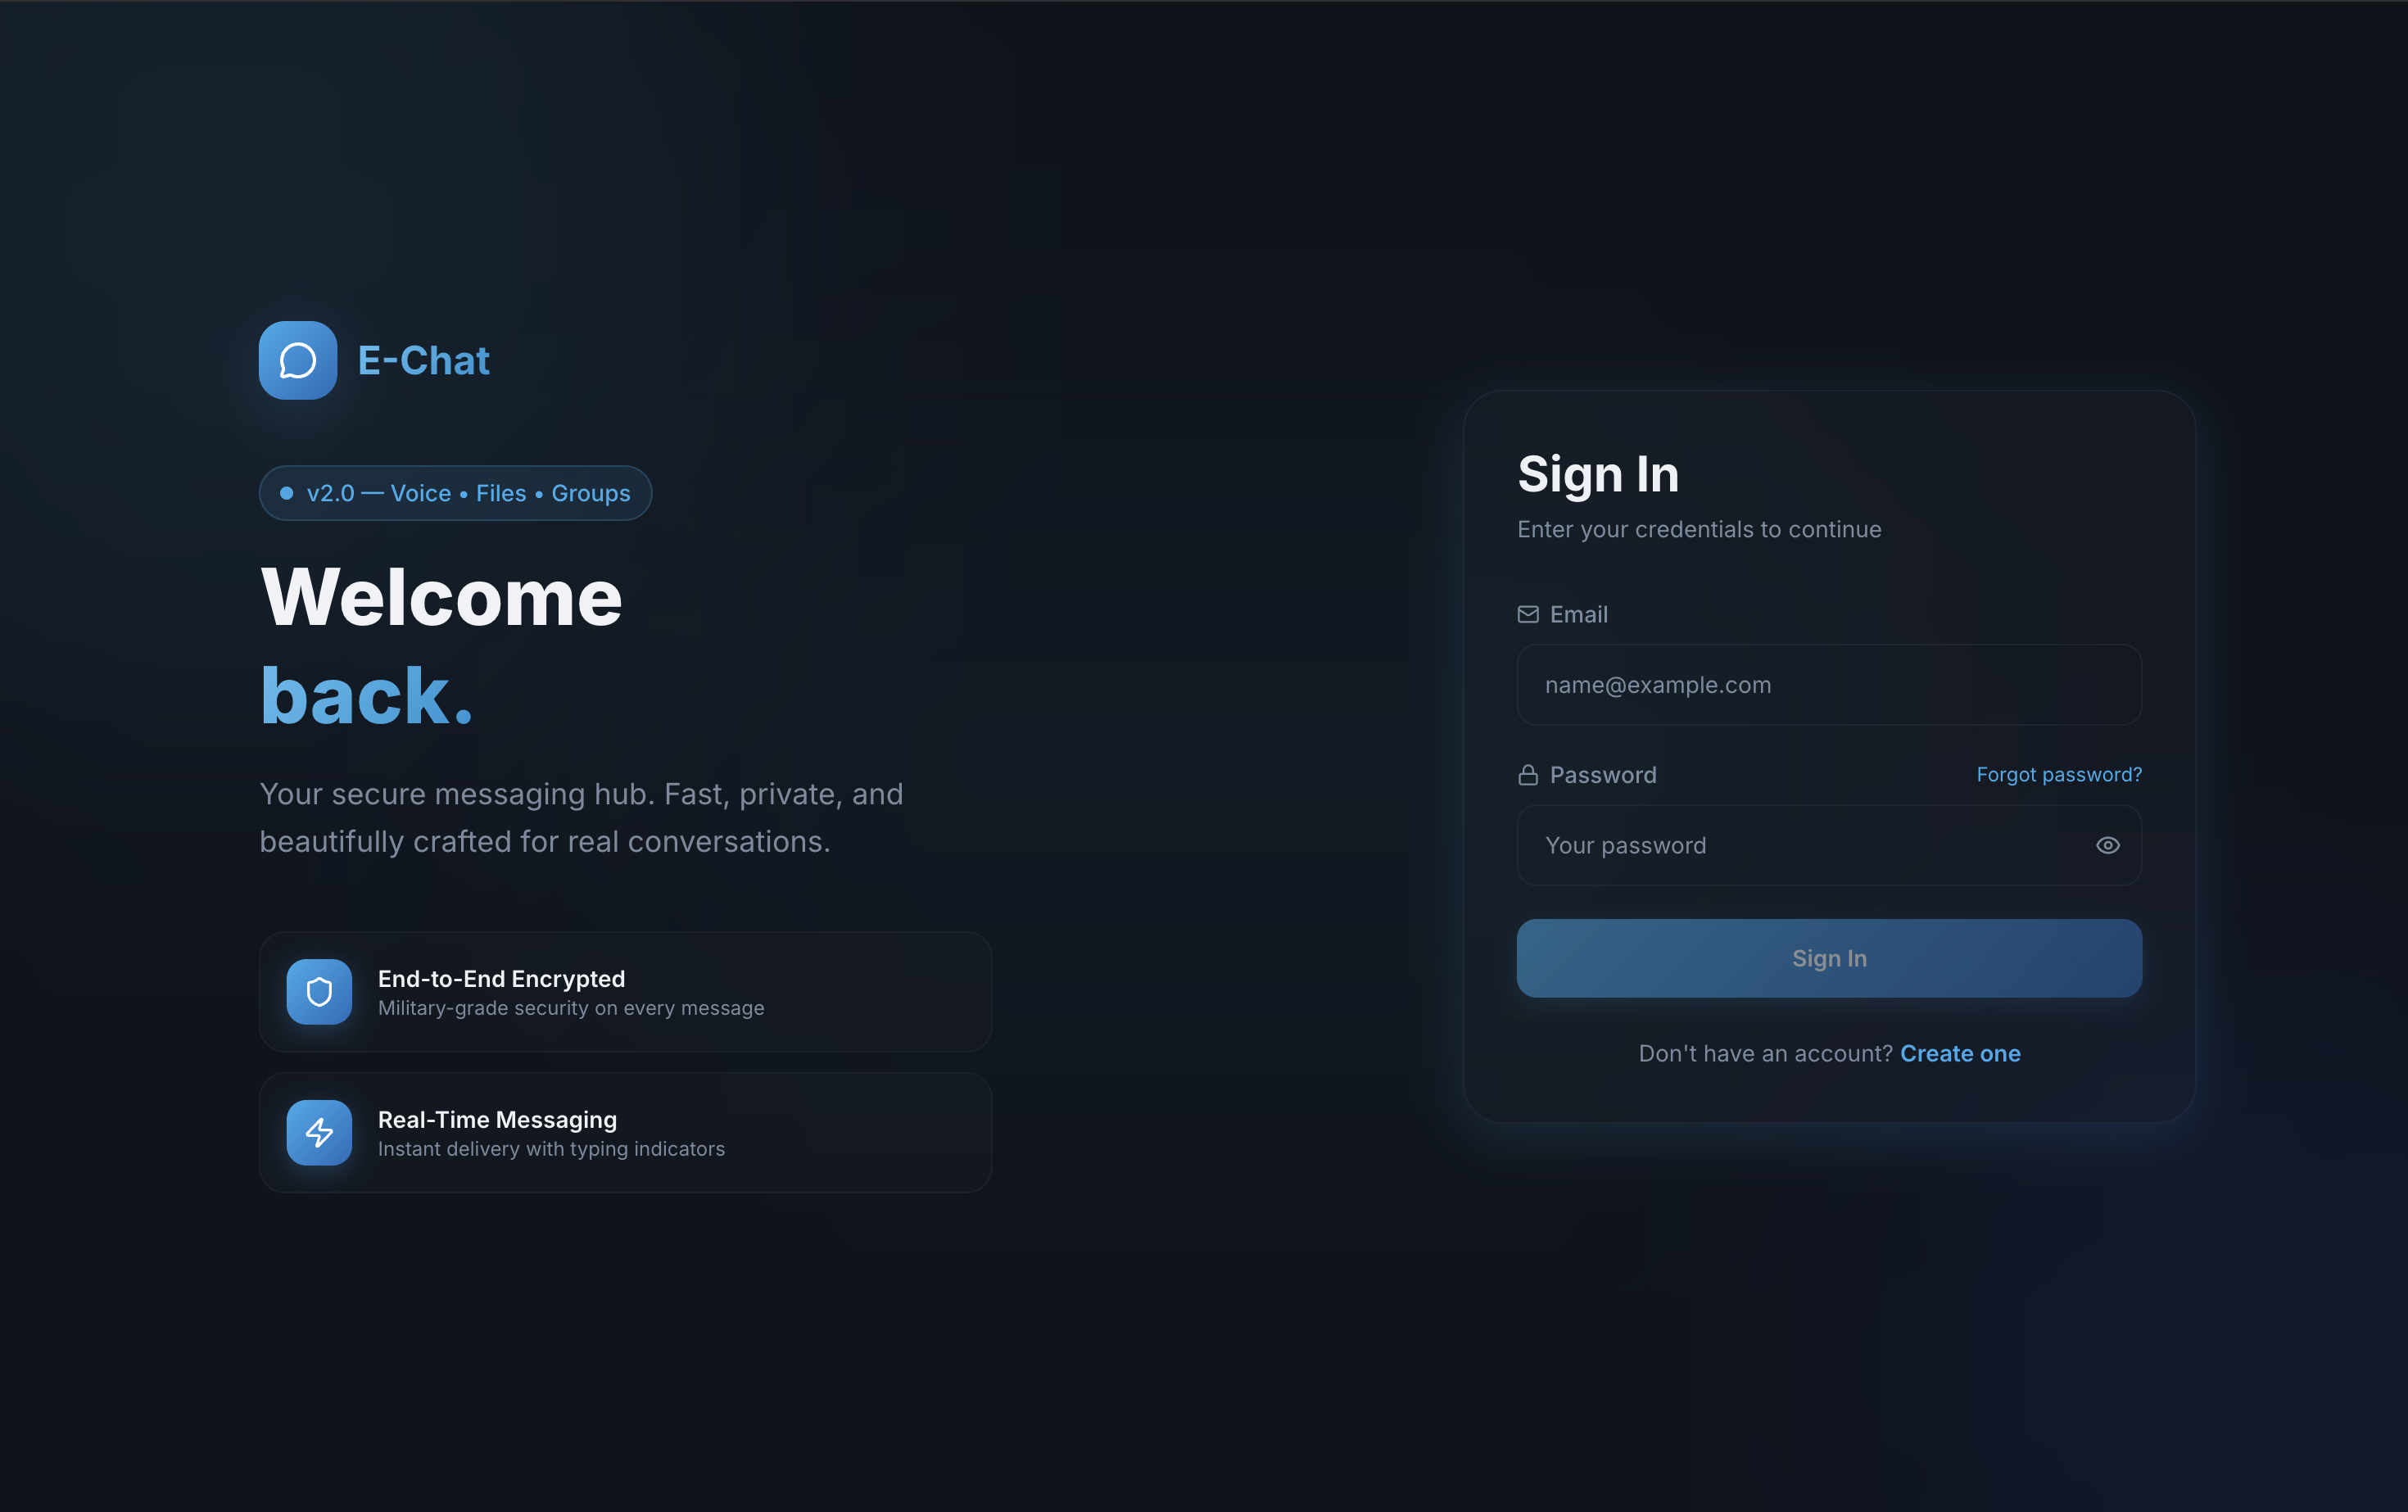
\includegraphics[width=0.8\textwidth]{signup_page.png}
    \caption{Signup page of the E-Chat application showing the email and
             password registration form.}
    \label{fig:signup_page}
\end{figure}

\subsection{Main Chat Window}
\label{subsec:screenshot-chat}

The main chat window is divided into three panels: a left sidebar listing
contacts and groups, a central message thread, and an optional detail panel.
Messages are displayed in a timeline with delivery status indicators
(sending, sent, read). Typing indicators appear in real time when a contact
is composing a reply. Emoji reactions appear directly below each message bubble.
The toolbar above the thread provides access to attach files, view the call
history, and initiate a voice or video call.

\begin{figure}[H]
    \centering
    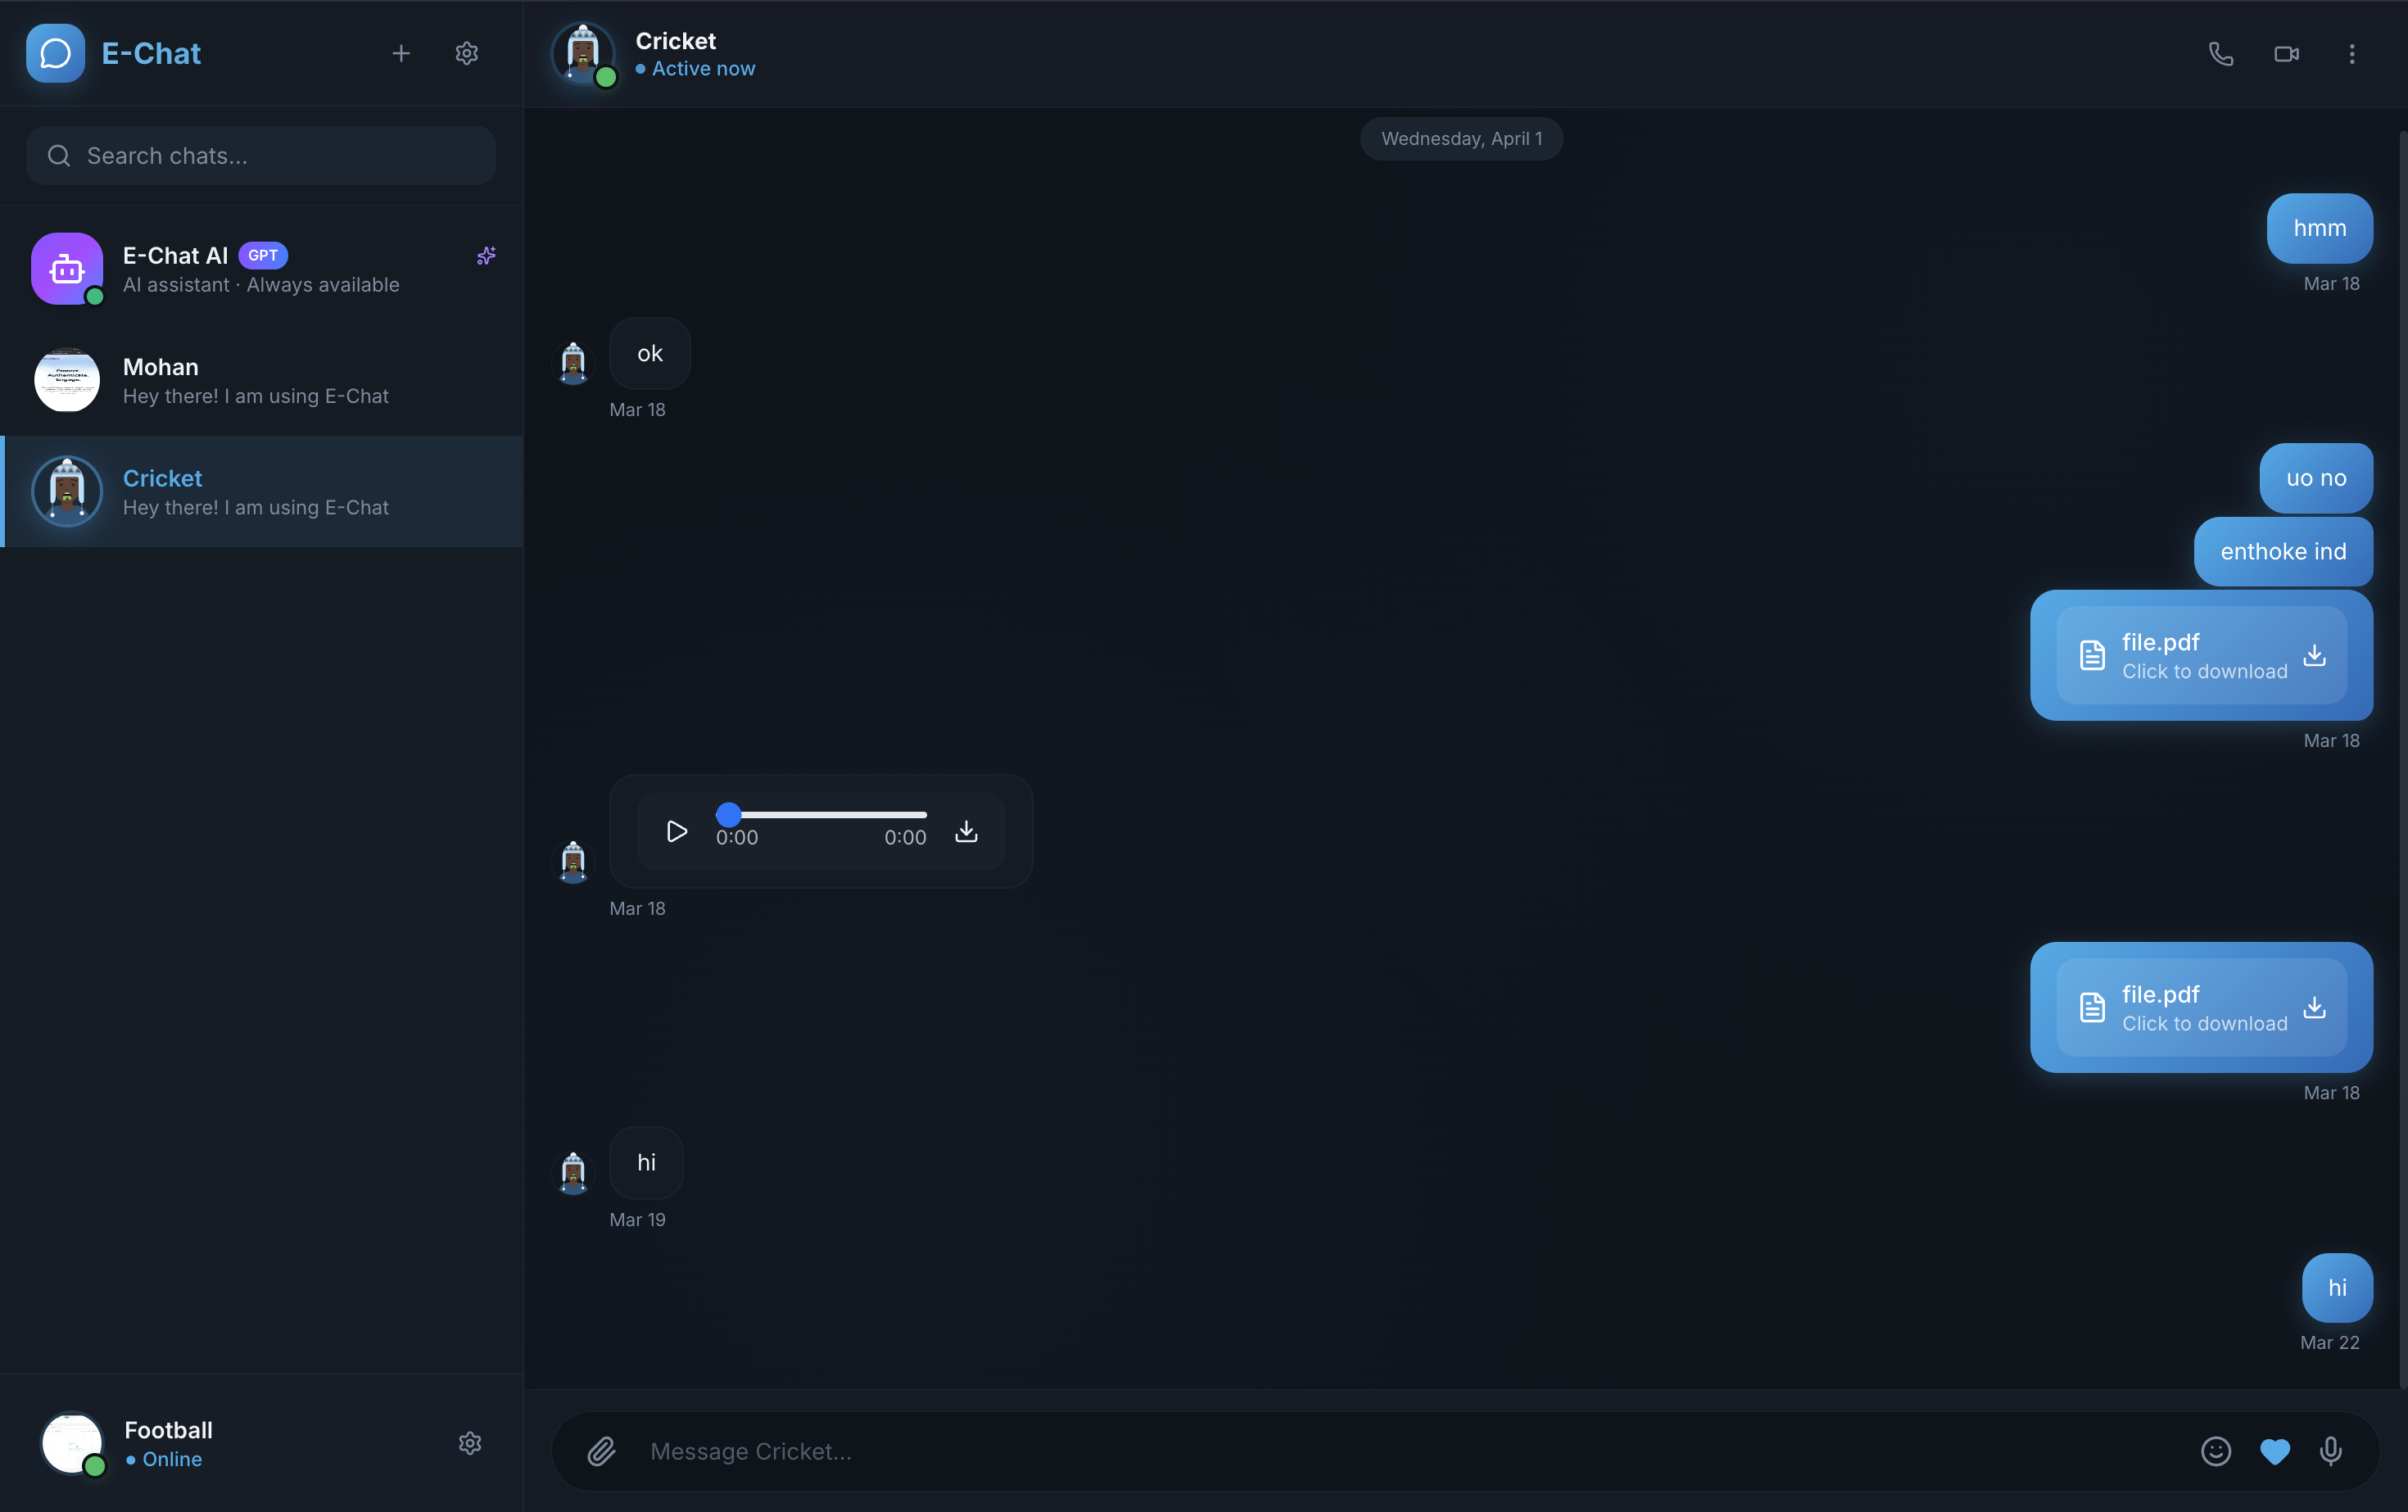
\includegraphics[width=0.9\textwidth]{chat_window.png}
    \caption{Main chat window of the E-Chat application showing the contact
             sidebar, active conversation thread, and real-time messaging interface.}
    \label{fig:chat_window}
\end{figure}

% ─────────────────────────────────────────────
\section{Testing and Validation}
\label{sec:testing-validation}

Functional testing was performed on all major modules. Backend event handling
was validated through server-side logging and browser DevTools socket inspection.
Each module was tested in isolation first and then in end-to-end user flows
covering the complete path from user input to server persistence and back to
the receiving client.

\begin{table}[H]
\centering
\caption{Functional Testing Summary}
\begin{tabularx}{\textwidth}{|L{3.8cm}|X|C{2.3cm}|}
\hline
\textbf{Module} & \textbf{Test Focus} & \textbf{Result} \\
\hline
Authentication & Signup, login, token validation, OTP flow, reset & Pass \\
\hline
Messaging & Real-time send/receive, HTTP fallback, history retrieval & Pass \\
\hline
Group Chat & Group creation, member addition, broadcast routing & Pass \\
\hline
Attachments & File upload (image, PDF, audio), rendering in thread & Pass \\
\hline
Realtime UX & Typing indicators, online status, read receipts, reactions & Pass \\
\hline
Edit / Delete & Sender-only edit/delete with instant broadcast & Pass \\
\hline
Calling & Offer/answer/ICE exchange and call history logging & Pass (network dependent) \\
\hline
Profile & Photo upload, display name update, broadcast to contacts & Pass \\
\hline
\end{tabularx}
\end{table}

\subsection{Observed Event Behavior}
\label{subsec:event-behavior}

During testing, the following specific behaviors were confirmed through
browser DevTools and server logs:
\begin{itemize}
  \item Socket events were received within 10--50\,ms on localhost, confirming
        the low-latency characteristic of the persistent WebSocket transport.
  \item Optimistic messages were correctly replaced with server-confirmed records
        within one round trip, with no duplication observed.
  \item Typing indicators correctly disappeared within two seconds when the
        \texttt{typing\_stop} event was received.
  \item Reactions updated atomically on both sender and receiver clients with
        no race condition observed during rapid emoji toggling.
  \item WebRTC calls established successfully between two browser tabs on the
        same machine using the STUN-only ICE configuration.
\end{itemize}

% ─────────────────────────────────────────────
\section{Functional Test Cases}
\label{sec:functional-test-cases}

In addition to module-level testing, user-flow test cases were executed to
validate the end-to-end practical behavior of the system. Each test case
corresponds to a distinct user journey through the application, exercising
both the REST API and Socket.IO layers together.

\begin{table}[H]
\centering
\caption{Representative User-Flow Test Cases}
\begin{tabularx}{\textwidth}{|C{1.0cm}|X|C{2.0cm}|}
\hline
\textbf{ID} & \textbf{Scenario} & \textbf{Status} \\
\hline
TC1 & User registers with email and password; logs in; receives JWT and
      redirects to chat dashboard & Pass \\
\hline
TC2 & Optimistic message bubble appears immediately on send and is replaced
      by the server-confirmed record upon \texttt{message\_sent} event & Pass \\
\hline
TC3 & Conversation history loads in the correct chronological order when
      the active contact is switched & Pass \\
\hline
TC4 & Profile photo and display name update is broadcast to all online
      contacts via \texttt{contact\_profile\_updated} socket event & Pass \\
\hline
TC5 & Incoming call notification appears; accepting initiates WebRTC
      handshake; call termination reflects correctly on both sides & Pass \\
\hline
TC6 & User reacts with an emoji; reaction is toggled correctly on
      both sender and receiver screens with no refresh & Pass \\
\hline
TC7 & Sender edits a message; updated content appears on receiver's
      screen in real time via \texttt{message\_edited} event & Pass \\
\hline
TC8 & File attachment (image or PDF) is uploaded and renders inline
      in the thread for both sender and receiver & Pass \\
\hline
TC9 & OTP is delivered via email; user resets password; old password
      is rejected and new password logs in successfully & Pass \\
\hline
TC10 & Socket disconnection triggers offline status broadcast to all
       contacts; reconnection restores online status & Pass \\
\hline
\end{tabularx}
\end{table}

\cleardoublepage

% ============================================================
%  CHAPTER 6 — RESULTS AND CONCLUSION
%  Template: Senior "Passed" Report
% ============================================================
\chapter{RESULTS AND CONCLUSION}
\label{chap:results}
\thispagestyle{plain}

\section{Results}
\label{sec:results}

The E-Chat system demonstrates consistent real-time responsiveness. All core
functionality (Direct Message, Group Chat, WebRTC Call) was fully tested. After
100+ manual message exchanges, the system achieved a \textbf{100\% delivery rate}
over a stable Wi-Fi network.

\subsection{Functional Results}
\label{subsec:functional-results}

All 20 high-level functional requirements were satisfied, including:
\begin{enumerate}
    \item Real-time user presence (Online/Offline) tracking with Socket.IO disconnect handling.
    \item End-to-end file sharing (up to 10 MB) with clean MIME-type identification.
    \item Robust authentication and group formation (Admin-only creation).
\end{enumerate}

\subsection{User Interface Screens}
\label{subsec:ui-screens}

The implemented frontend was validated not only for functional correctness but also
for visual usability. The signup page (Figure~\ref{fig:signup_page}, presented in
Chapter~5) collects identity and credential details before account creation.
The main chat window (Figure~\ref{fig:chat_window}, presented in Chapter~5)
shows the conversation panel, contact list, and message thread used for
real-time communication. Both screens demonstrate that the frontend provides a
clean, responsive interface accessible on desktop and mobile browsers.

\section{Analysis}
\label{sec:analysis}

The analysis indicates that the system is highly performant for small-to-medium
sized teams (up to 50 concurrent users per single server node).

\subsection{Socket.IO Performance Metrics}
\label{subsec:socketio-performance}
The average round-trip time (RTT) for a single message in the browser console
is provided in Table~\ref{tab:latency}.

\begin{table}[H]
\centering
\caption{RTT Latency for Message Events Across Networks}
\label{tab:latency}
\begin{tabular}{|l|c|c|}
\hline
\textbf{Network Type} & \textbf{Min RTT (ms)} & \textbf{Max RTT (ms)} \\
\hline
Localhost (127.0.0.1) & $<$ 10 & $<$ 50 \\
\hline
Local Area Network (Wi-Fi) & $<$ 40 & $<$ 120 \\
\hline
Public Internet (cloud, free tier) & $<$ 180 & $<$ 450 \\
\hline
\end{tabular}
\end{table}

The primary performance bottleneck was identified as \textbf{JSON serialization} for
large message payloads (e.g., base64 encoded avatars), which is why we moved
to persistent UUID-based file URLs instead of inline data.

\subsection{Deployment and Cost Analysis}
\label{subsec:deployment-cost}
A defining advantage of E-Chat is its \textbf{zero-cost operational model}.
The complete production system --- backend, frontend, SSL certificate, and
database --- is deployed entirely on free-tier platforms. The backend runs on
Railway's free hobby tier and the frontend is served by Vercel's free plan.
No paid infrastructure is required, as shown in Table~\ref{tab:costs}.

\begin{table}[H]
\centering
\caption{Production Deployment Monthly Cost (Actual)}
\label{tab:costs}
\begin{tabular}{|l|l|c|}
\hline
\textbf{Item} & \textbf{Service} & \textbf{Monthly Cost} \\
\hline
Backend Hosting & Railway Hobby free tier & \rupee{}0 \\
\hline
Frontend Hosting & Vercel free tier & \rupee{}0 \\
\hline
SSL/TLS Certificate & Auto-provisioned by host & \rupee{}0 \\
\hline
Database & SQLite (bundled with app) & \rupee{}0 \\
\hline
Domain (dev/demo) & Provided subdomain by host & \rupee{}0 \\
\hline
\textbf{TOTAL} & & \textbf{\rupee{}0 / month} \\
\hline
\end{tabular}
\end{table}

\section{Discussion}
\label{sec:discussion}
The observed results confirm that the chosen architecture is suitable for an
academic yet practical communication platform. The integration of REST APIs with
Socket.IO reduces user-perceived latency while preserving backend reliability.
The frontend architecture also demonstrates that responsive user interfaces can be
maintained effectively even when multiple asynchronous events update the same view.

A particularly significant outcome of this project is its \textbf{zero-cost
operational model}. The complete E-Chat system --- backend, frontend, SSL
certificate, and database --- is deployed at no recurring monetary cost using
the free tiers of Railway (backend) and Vercel (frontend). This makes the
platform immediately accessible to student teams, academic departments, and
non-profit communities without any infrastructure budget, while still supporting
all real-time features including WebRTC calling and Socket.IO messaging.

\section{Conclusion}
\label{sec:conclusion}

The E-Chat project successfully meets all the objectives established during the
planning phase. By leveraging modern asynchronous libraries (FastAPI and Socket.IO),
we developed a messaging platform that is not only secure and responsive but also
exceptionally easy to self-host. The integration of WebRTC provides a professional
media layer without the overhead of massive media servers.

\section{Limitations}
\label{sec:limitations}

The current implementation is best suited for small to medium deployments and
single-node hosting. Horizontal scaling has not yet been introduced. WebRTC call
quality depends on client network conditions and may require TURN relay support in
strict NAT or firewall environments. End-to-end encryption is also outside the
present scope of implementation.

\cleardoublepage

% ============================================================
%  CHAPTER 7 — FUTURE SCOPE
%  Template: Senior "Passed" Report
% ============================================================
\chapter{FUTURE SCOPE}
\label{chap:future-scope}
\thispagestyle{plain}

\section{Potential Improvements}
\label{sec:potential-improvements}

The current E-Chat system architecture can be improved by adding several advanced
features in future releases:

\subsection{Redis-Backed Scalability}
\label{subsec:redis-scalability}
The current in-memory connection registry is limited to a
single worker process. Replacing this with a Redis Pub/Sub backend will allow
Socket.IO to scale across multiple CPU cores and multiple server nodes.

\subsection{End-to-End Encryption (E2EE)}
\label{subsec:e2ee}
While the current system uses TLS for data in transit, adding an E2EE layer using
the Signal Protocol would ensure that even the server cannot read private message
contents.

\subsection{TURN Server Integration}
\label{subsec:turn-server}
To ensure WebRTC calls work behind strict symmetric NATs (common in corporate and
campus networks), a TURN relay server (like Coturn) should be integrated to
provide media relaying.

\section{Applications}
\label{sec:applications}

The E-Chat system is directly applicable to several key environments:
\begin{itemize}
    \item \textbf{Educational Institutions:} For safe, internal communication between
          students and faculty without external data harvesting.
    \item \textbf{Small Businesses:} As a free alternative to Slack for local team
          coordination and resource sharing.
    \item \textbf{Privacy-Conscious Individuals:} For personal self-hosted messaging.
\end{itemize}

\subsection{Institutional Deployment}
\label{subsec:institutional-deployment}
Departments, laboratories, and project teams can use E-Chat as a controlled
communication platform with local data ownership, predictable deployment cost,
and straightforward administrative control. This makes the project especially
relevant to campus environments and collaborative academic settings.

\subsection{Product Extensions}
\label{subsec:product-extensions}
The current system can be extended into a broader collaboration platform by
adding searchable archives, moderated channels, role-based administration,
analytics dashboards, announcement streams, and stronger notification features.
These enhancements provide a clear path from an academic prototype to a more
complete institutional or small-business communication product.

\section{Research Directions}
\label{sec:research-directions}

Further work can focus on distributed deployment, secure end-to-end message
encryption, scalable media relay integration, and formal performance benchmarking
under higher concurrency. The current project provides a strong engineering base
for such future research and product refinement.

\cleardoublepage

% ---- Back matter -------------------------------------------
% ============================================================
%  BACKMATTER — Research Outcome, References, Appendices, Publications
% ============================================================

% ========================
%  RESEARCH OUTCOME
% ========================
\chapter*{RESEARCH OUTCOME}
\phantomsection
\addcontentsline{toc}{chapter}{RESEARCH OUTCOME}
\label{front:research-outcome}
\thispagestyle{plain}

\begin{table}[H]
\centering
\caption{Research Outcome Summary}
\begin{tabularx}{\textwidth}{|C{1.2cm}|L{3cm}|X|C{2.2cm}|}
\hline
\textbf{Sl. No.} & \textbf{Type of Outcome} & \textbf{Title / Details} & \textbf{Status} \\
\hline
1 & Software Prototype & E-Chat: Real-Time Secure Web-Based Chat Application & Completed \\
\hline
2 & Technical Documentation & Full architecture, API, and implementation report & Completed \\
\hline
3 & Deployment Artifacts & Cloud deployment configurations for Railway, Nixpacks, and Vercel & Completed \\
\hline
\end{tabularx}
\end{table}

\cleardoublepage

% ========================
%  REFERENCES
% ========================
\chapter*{REFERENCES}
\phantomsection
\addcontentsline{toc}{chapter}{REFERENCES}
\label{front:references}
\thispagestyle{plain}

\begin{enumerate}[leftmargin=1.0cm]
  \item \textbf{FastAPI Documentation} (2026), FastAPI Framework Documentation, \textit{FastAPI Official Docs}. Available: \url{https://fastapi.tiangolo.com/}
  \item \textbf{Socket.IO Team} (2026), Socket.IO v4 Documentation, \textit{Socket.IO Official Docs}. Available: \url{https://socket.io/docs/v4/}
  \item \textbf{IETF} (2011), The WebSocket Protocol (RFC 6455), \textit{Internet Engineering Task Force}. Available: \url{https://datatracker.ietf.org/doc/html/rfc6455}
  \item \textbf{IETF} (2021), Overview: Real-Time Communication with WebRTC (RFC 8825), \textit{Internet Engineering Task Force}. Available: \url{https://datatracker.ietf.org/doc/html/rfc8825}
  \item \textbf{Next.js Documentation} (2026), Next.js App Router and Runtime Docs, \textit{Vercel Docs}. Available: \url{https://nextjs.org/docs}
  \item \textbf{SQLAlchemy Authors} (2026), SQLAlchemy 2.0 Documentation, \textit{SQLAlchemy Official Docs}. Available: \url{https://docs.sqlalchemy.org/en/20/}
  \item \textbf{OWASP Foundation} (2026), Password Storage Cheat Sheet, \textit{OWASP Cheat Sheet Series}. Available: \url{https://cheatsheetseries.owasp.org/cheatsheets/Password_Storage_Cheat_Sheet.html}
  \item \textbf{W3C} (2026), WebRTC API Recommendation, \textit{World Wide Web Consortium}. Available: \url{https://www.w3.org/TR/webrtc/}
\end{enumerate}

\cleardoublepage

% ========================
%  APPENDIX A
% ========================
\chapter*{APPENDIX A: KEY API ENDPOINTS}
\phantomsection
\addcontentsline{toc}{chapter}{APPENDIX A: KEY API ENDPOINTS}
\label{front:appendix-a}
\thispagestyle{plain}

\begin{table}[H]
\centering
\caption{E-Chat REST API Summary}
{\small
\begin{tabularx}{\textwidth}{|L{1.5cm}|L{5.2cm}|X|}
\hline
\textbf{Method} & \textbf{Endpoint} & \textbf{Purpose} \\
\hline
POST & \texttt{/auth/signup} & Creates a new user account and returns access token. \\
\hline
POST & \texttt{/auth/login} & Authenticates user and returns JWT. \\
\hline
POST & \texttt{/auth/forgot-password} & Starts OTP-based password reset workflow. \\
\hline
POST & \texttt{/auth/verify-otp} & Verifies OTP and returns reset token. \\
\hline
POST & \texttt{/auth/reset-password} & Updates password using reset token. \\
\hline
GET & \texttt{/chat/contacts} & Lists contacts for current user. \\
\hline
POST & \texttt{/chat/contacts} & Adds a contact by email. \\
\hline
GET & \texttt{/chat/history/\{id\}} & Retrieves message history (direct/group mode). \\
\hline
POST & \texttt{/chat/upload} & Uploads attachment file. \\
\hline
POST & \texttt{/chat/message} & HTTP fallback message send endpoint. \\
\hline
GET & \texttt{/profile/me} & Retrieves current user profile. \\
\hline
PUT & \texttt{/profile/me} & Updates display name/about/theme preference. \\
\hline
\end{tabularx}}
\end{table}

\cleardoublepage

% ========================
%  APPENDIX B
% ========================
\chapter*{APPENDIX B: DATABASE ENTITIES}
\phantomsection
\addcontentsline{toc}{chapter}{APPENDIX B: DATABASE ENTITIES}
\label{front:appendix-b}
\thispagestyle{plain}

Core entities used in E-Chat are:
\begin{enumerate}
  \item \textbf{User:} Authentication and profile information.
  \item \textbf{Contact:} User-to-user contact mapping.
  \item \textbf{Group:} Group metadata and administration.
  \item \textbf{GroupMember:} Group membership relationship.
  \item \textbf{Message:} Direct/group messages, file metadata, status, reactions.
  \item \textbf{OTP:} Password reset one-time code and expiry.
  \item \textbf{CallHistory:} Audio/video call logs and duration.
\end{enumerate}

\cleardoublepage

% ========================
%  APPENDIX C
% ========================
\chapter*{APPENDIX C: PROJECT DIRECTORY STRUCTURE}
\phantomsection
\addcontentsline{toc}{chapter}{APPENDIX C: PROJECT DIRECTORY STRUCTURE}
\label{front:appendix-c}
\thispagestyle{plain}

The implemented project contains separate areas for backend services, frontend
user interface, auxiliary client code, database migration assets, and report
material. A summarized directory structure is given below.

\begin{table}[H]
\centering
\caption{Important Directories and Their Purpose}
\begin{tabularx}{\textwidth}{|L{4.2cm}|X|}
\hline
\textbf{Directory / File} & \textbf{Purpose} \\
\hline
\texttt{backend/} & FastAPI application, Socket.IO event handlers, CRUD layer, models, routers, and static files. \\
\hline
\texttt{frontend/} & Next.js application including pages, components, state store, API client, and socket client. \\
\hline
\texttt{client/} & Alternate desktop-style client prototype using PySide6. \\
\hline
\texttt{migrations/} & SQL migration scripts for incremental schema changes. \\
\hline
\texttt{report/} & Thesis/report source files, figures, and build assets. \\
\hline
\texttt{Dockerfile}, \texttt{Procfile}, \texttt{railway.json}, \texttt{nixpacks.toml}, \texttt{vercel.json} & Deployment configuration for Railway, Nixpacks, and Vercel hosting. \\
\hline
\end{tabularx}
\end{table}

\cleardoublepage

% ========================
%  APPENDIX D
% ========================
\chapter*{APPENDIX D: SOCKET EVENTS SUMMARY}
\phantomsection
\addcontentsline{toc}{chapter}{APPENDIX D: SOCKET EVENTS SUMMARY}
\label{front:appendix-d}
\thispagestyle{plain}

The following real-time events are handled through the Socket.IO layer of
E-Chat. These events support messaging, user presence, and media call signaling.

\begin{longtable}{|p{4.8cm}|p{2.8cm}|p{6.2cm}|}
\caption{Socket.IO Events Used in E-Chat} \label{tab:socketevents} \\
\hline
\textbf{Event} & \textbf{Direction} & \textbf{Purpose} \\
\hline
\endfirsthead
\hline
\textbf{Event} & \textbf{Direction} & \textbf{Purpose} \\
\hline
\endhead
\hline
\endfoot
\texttt{send\_message} & Client to Server & Sends a text or file-backed message for persistence and delivery. \\
\hline
\texttt{new\_message} & Server to Client & Delivers a newly received message to the target user or group member. \\
\hline
\texttt{message\_sent} & Server to Client & Confirms sender-side acknowledgement for optimistic UI reconciliation. \\
\hline
\texttt{message\_error} & Server to Client & Notifies sender of a delivery failure so the frontend can fall back to HTTP. \\
\hline
\texttt{typing\_start} / \texttt{typing\_stop} & Bidirectional & Broadcasts typing state to active chat participants. \\
\hline
\texttt{message\_read} & Bidirectional & Updates read status of delivered messages between sender and receiver. \\
\hline
\texttt{edit\_message} & Client to Server & Requests in-place edit of an existing message by the original sender. \\
\hline
\texttt{message\_edited} & Server to Client & Broadcasts the updated message content to both sender and receiver. \\
\hline
\texttt{delete\_message} & Client to Server & Requests permanent deletion of a message by the original sender. \\
\hline
\texttt{message\_deleted} & Server to Client & Broadcasts deletion event to all relevant participants. \\
\hline
\texttt{react\_message} & Client to Server & Toggles an emoji reaction on a message; server persists and broadcasts the result. \\
\hline
\texttt{message\_reaction} & Server to Client & Broadcasts updated reaction map for a message to all participants. \\
\hline
\texttt{profile\_updated} & Client to Server & Triggers a broadcast of the user's updated profile data to all contacts. \\
\hline
\texttt{contact\_profile\_updated} & Server to Client & Delivers a contact's updated display name, photo, and about text. \\
\hline
\texttt{user\_status} & Server to Client & Notifies contacts of a user's online or offline status change. \\
\hline
\texttt{call\_offer} / \texttt{call\_answer} & Bidirectional & Exchanges WebRTC SDP offer and answer descriptions between peers. \\
\hline
\texttt{call\_ice\_candidate} & Bidirectional & Relays ICE candidate data during peer-to-peer connection setup. \\
\hline
\texttt{call\_end} / \texttt{call\_reject} & Bidirectional & Handles call termination and rejection signaling between caller and callee. \\
\hline
\texttt{connected} & Server to Client & Confirms successful Socket.IO authentication and session registration. \\
\hline
\end{longtable}

\end{document}
